%%%%%%%%%%%%%%%%%%%%%%%%%%%%%%%%%%%
%06f Syntax ue-loesung03
%%%%%%%%%%%%%%%%%%%%%%%%%%%%%%%%%%%
	
\begin{frame}
\frametitle{Übung -- Lösung}


\begin{columns}

\begin{column}{.45\textwidth}
\begin{figure}
	\scalebox{.6}{\begin{forest} sm edges,
			[S
			[VP [V [Tea] ] ]
			[NP
			[P [with]]
			[Det [some]]
			[N [lemon]]
			]
			[PP
			[P [tastes]]
			[NP [Adj [really] ] [N [nice]] ]
			]
			]
	\end{forest}}
	%	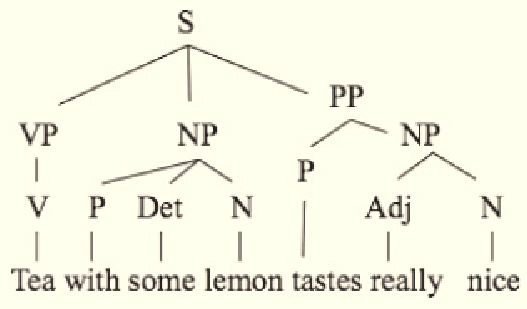
\includegraphics[scale=.45]{material/wrongtree}
	\caption{vgl.\ \url{http://specgram.com/CLXV.1/05.cruz-ferreira.know22.html}}
\end{figure}
\end{column}
%%
%%
\begin{column}{.55\textwidth}

\begin{itemize}
	\alertgreen{\item keine binäre Struktur (mehr als zwei Töchter)}
	\alertgreen{\item falsche Kategorien bestimmt (\zB \MyPobj{Tea}: V?)}
	\alertgreen{\item Es gibt Köpfe ohne Phrasen}
	\alertgreen{\item keine Zwischen Projektionen}
	\alertgreen{\item Satz ist exozentrisch}
	\alertgreen{\item \dots}
\end{itemize}

\end{column}
\end{columns}

\end{frame}
